%\newpage

\section{Experiments}
\label{sec:experiments}

Experiments have been performed by trying input sizes of different lengths.
For each length $k$, a sample of 1000000 random numbers was generated in the interval $[2^{k-1}, 2^k>$ and for these numbers we recorded the runtime and the fraction of samples that was predicted correctly.
    For AKS these experiments had to be aborted at a certain point, because this algorithm turned out to be very slow.

\subsection{Measurements}
Since all the probablitic algorithm have a one-sided error, we decided to look at the probability that a number classified as prime is actually prime.
So we tried to estimate $Pr(\text{x is prime} | \text{x is detected as prime}$.
This probability can be approximated by $E = \frac{FP}{TP + FP}$, where TP is the number of prime numbers that are classified correctly and FP is the number of non-primes to be classified as prime.
So in the experiments we used $E$ as an error measure.

\section{Results}
\label{sec:results}

We can see the runtime in Table \ref{table:runtime} and we can see the runtime plotted in Figure \ref{fig:runtime}.

As we see the Trial Divion and Wheel Sieve algorithm perform well for small data, but for big numbers they are exponential in the input size.
As these algorithms are deterministic, the error rate on these numbers is $0\%$.

For bigger data SS and MR perform better in execution time.
MR seems to outperform SS both in runtime and in error rate.
However for the runtime this might depend on how we implemented those since theoretically both have about the same time complexity.

Although AKS would theoretically run in polynomial time, it really is the snail of the bunch and therefore it has been decided to drop the results for integers above $2^{13}$.
In the runtime graph, the line for AKS is almost a straight vertical line.
It appears that AKS is especially slow when it's running on a number that is prime.
We performed an additional test of AKS on numbers in the range 2 - 500 and noticed that for composite numbers, the algorithm generally finished in less than a second, but when ran on both prime and composite numbers, the algorithm could last up to $10e9$s.
This has been summarized in Table \ref{tab:pressure}.

Something else that looks interesting is that for the probablistic methods the error is low for both small and large inputs.
For small inputs, this is probably because there are many small primes numbers and for prime numbers these tests never fail. %more random numbers for which the SS and MR tests succeed.
For large inputs the error is probably small, because large numbers are more likely to have many divisors and therefore the algorithms might be more likely to pick a random number that has factors in common with those big numbers.
%, primes get more rare and it is more likely that the algorithm is being tested on a lot of composite numbers.

\begin{table}
    \centering
    \caption{Execution time as a function of $\log n$ in milliseconds}
    \begin{tabular}{|l|c|c|c|c|c|} \hline
        $\log n$ & SS & AKS & MR & TD & WS \\
        \hline
1 & 7 & 433039 & 10 & 8 & 8 \\
2 & 105 & 3013323 & 108 & 30 & 8 \\
3 & 95 & 5205242 & 115 & 16 & 12 \\
4 & 108 & 192011802 & 123 & 22 & 13 \\
5 & 142 & 163575911 & 162 & 25 & 17 \\
6 & 156 & 926665397 & 165 & 28 & 17 \\
7 & 183 & 3786175634 & 186 & 32 & 19 \\
8 & 200 & 9929344339 & 195 & 37 & 19 \\
9 & 225 & 20959122837 & 214 & 40 & 21 \\
10 & 246 & 45109241251 & 222 & 46 & 24 \\
11 & 267.0 & - & 241.0 & 54.0 & 27.0 \\
12 & 291.0 & - & 252.0 & 64.0 & 30.0 \\
13 & 347.0 & - & 262.0 & 79.0 & 35.0 \\
14 & 354.0 & - & 274.0 & 94.0 & 40.0 \\
15 & 352.0 & - & 286.0 & 115.0 & 48.0 \\
16 & 374.0 & - & 346.0 & 142.0 & 57.0 \\
17 & 399.0 & - & 313.0 & 181.0 & 75.0 \\
18 & 424.0 & - & 318.0 & 230.0 & 87.0 \\
19 & 438.0 & - & 331.0 & 295.0 & 109.0 \\
20 & 467.0 & - & 340.0 & 383.0 & 140.0 \\
21 & 479.0 & - & 352.0 & 504.0 & 178.0 \\
22 & 501.0 & - & 364.0 & 665.0 & 232.0 \\
23 & 547.0 & - & 376.0 & 877.0 & 303.0 \\
24 & 545.0 & - & 388.0 & 1180.0 & 404.0 \\
25 & 569.0 & - & 401.0 & 1614.0 & 540.0 \\
26 & 588.0 & - & 414.0 & 2116.0 & 722.0 \\
27 & 611.0 & - & 425.0 & 2846.0 & 965.0 \\
28 & 633.0 & - & 438.0 & 3871.0 & 1296.0 \\
29 & 660.0 & - & 449.0 & 5212.0 & 1743.0 \\
30 & 670.0 & - & 462.0 & 7069.0 & 2371.0 \\
31 & 694.0 & - & 477.0 & 9595.0 & 3212.0 \\
%1 & 8 & 1726 & 13 & 12 & 8 \\
%2 & 110 & 19326 & 128 & 8 & 8 \\
%3 & 110 & 32415 & 130 & 14 & 16 \\
%4 & 122 & 689248 & 140 & 20 & 14 \\
%5 & 156 & 582623 & 184 & 23 & 18 \\
%6 & 169 & 3735301 & 190 & 26 & 18 \\
%7 & 192 & 10045207 & 212 & 29 & 20 \\
%8 & 211 & 21503625 & 217 & 32 & 21 \\
%9 & 234 & 60103404 & 237 & 36 & 22 \\
%10& 254 & 127910717 & 245 & 40 & 25 \\
%11& 275 & 292019772 & 256 & 46 & 27 \\
%12& 297 & 581977224 & 269 & 54 & 30 \\
%13& 321 & 1014476731 & 278 & 64 & 34 \\
%14& 726.0 & - & 292.0 & 78.0 & 39.0 \\
%15& 1278.0 & - & 304.0 & 94.0 & 44.0 \\
%16& 702.0 & - & 316.0 & 117.0 & 52.0 \\
%17& 749.0 & - & 330.0 & 149.0 & 63.0 \\
%18& 790.0 & - & 342.0 & 189.0 & 77.0 \\
%19& 830.0 & - & 354.0 & 251.0 & 94.0 \\
%20& 873.0 & - & 369.0 & 325.0 & 118.0 \\
%21& 914.0 & - & 382.0 & 1499.0 & 154.0 \\
%22& 954.0 & - & 409.0 & 1005.0 & 513.0 \\
%23& 997.0 & - & 747.0 & 1332.0 & 727.0 \\
%24& 1037.0 & - & 772.0 & 1798.0 & 624.0 \\
%25& 1075.0 & - & 794.0 & 2399.0 & 828.0 \\
%26& 1120.0 & - & 819.0 & 3252.0 & 1112.0 \\
%27& 1157.0 & - & 844.0 & 4438.0 & 1512.0 \\
%28& 1197.0 & - & 871.0 & 6130.0 & 2073.0 \\
%29& 1238.0 & - & 897.0 & 7479.0 & 2841.0 \\
%30& 1017.0 & - & 922.0 & 11676.0 & 3915.0 \\
%31& 1318.0 & - & 947.0 & 14595.0 & 5036. \\
        \hline
    \end{tabular}
    \label{table:runtime}
\end{table}


\begin{table}
    \centering
    \caption{Error as a function of $\log n$}
    \begin{tabular}{|l|c|c|c|c|c|} \hline
        $\log n$ & SS & AKS & MR & TD & WS \\
        \hline
1 & 0 & 0 & 0 & 0 & 0 \\
2 & 0 & 0 & 0 & 0 & 0 \\
3 & 0 & 0 & 0 & 0 & 0 \\
4 & 0.1638 & 0 & 0.1644 & 0 & 0 \\
5 & 0.06474 & 0 & 0.06485 & 0 & 0 \\
6 & 0.07124 & 0 & 0.0655 & 0 & 0 \\
7 & 0.0659 & 0 & 0.05616 & 0 & 0 \\
8 & 0.04387 & 0 & 0.03831 & 0 & 0 \\
9 & 0.03733 & 0 & 0.0312 & 0 & 0 \\
10 & 0.02583 & 0 & 0.02086 & 0 & 0 \\
11 & 0.02454 & - & 0.01775 & 0 & 0 \\
12 & 0.01608 & - & 0.01056 & 0 & 0 \\
13 & 0.01065 & - & 0.008065 & 0 & 0 \\
14 & 0.008712 & - & 0.006069 & 0 & 0 \\
15 & 0.005533 & - & 0.003722 & 0 & 0 \\
16 & 0.004698 & - & 0.002742 & 0 & 0 \\
17 & 0.002837 & - & 0.001715 & 0 & 0 \\
18 & 0.002124 & - & 0.001372 & 0 & 0 \\
19 & 0.001626 & - & 0.0009099 & 0 & 0 \\
20 & 0.001303 & - & 0.00072 & 0 & 0 \\
21 & 0.0009645 & - & 0.0005392 & 0 & 0 \\
22 & 0.0005828 & - & 0.0002242 & 0 & 0 \\
23 & 0.0003461 & - & 0.0001259 & 0 & 0 \\
24 & 0.0003897 & - & 0.0001624 & 0 & 0 \\
25 & 0.0001196 & - & 0.0001367 & 0 & 0 \\
26 & 7.101e-05 & - & 7.101e-05 & 0 & 0 \\
27 & 9.212e-05 & - & 1.843e-05 & 0 & 0 \\
28 & 5.69e-05 & - & 1.897e-05 & 0 & 0 \\
29 & 3.964e-05 & - & 0 & 0 & 0 \\
30 & 2.049e-05 & - & 0 & 0 & 0 \\
31 & 4.25e-05 & - & 0 & 0 & 0 \\
%1 & 1.0 & 1.0 & 1.0 & 1.0 & 1.0 \\
%2 & 1.0 & 1.0 & 1.0 & 1.0 & 1.0 \\
%3 & 1.0 & 1.0 & 1.0 & 1.0 & 1.0 \\
%4 & 0.951203 & 1.0 & 0.95053 & 1.0 & 1.0 \\
%5 & 0.978582 & 1.0 & 0.978538 & 1.0 & 1.0 \\
%6 & 0.983269 & 1.0 & 0.984793 & 1.0 & 1.0 \\
%7 & 0.985784 & 1.0 & 0.987807 & 1.0 & 1.0 \\
%8 & 0.991804 & 1.0 & 0.992822 & 1.0 & 1.0 \\
%9 & 0.993558 & 1.0 & 0.99467 & 1.0 & 1.0 \\
%10& 0.995892 & 1.0 & 0.996872 & 1.0 & 1.0 \\
%11& 0.996757 & 1.0 & 0.997659 & 1.0 & 1.0 \\
%12& 0.997884 & 1.0 & 0.998644 & 1.0 & 1.0 \\
%13& 0.998752 & 1.0 & 0.999046 & 1.0 & 1.0 \\
%14& 0.999077 & - & 0.999402 & 1.0 & 1.0 \\
%15& 0.999396 & - & 0.999603 & 1.0 & 1.0 \\
%16& 0.999572 & - & 0.999767 & 1.0 & 1.0 \\
%17& 0.999736 & - & 0.999844 & 1.0 & 1.0 \\
%18& 0.999832 & - & 0.999898 & 1.0 & 1.0 \\
%19& 0.999872 & - & 0.999928 & 1.0 & 1.0 \\
%20& 0.999923 & - & 0.999947 & 1.0 & 1.0 \\
%21& 0.99994 & - & 0.999969 & 1.0 & 1.0 \\
%22& 0.999975 & - & 0.999988 & 1.0 & 1.0 \\
%23& 0.999971 & - & 0.999994 & 1.0 & 1.0 \\
%24& 0.999983 & - & 0.99999 & 1.0 & 1.0 \\
%25& 0.999991 & - & 0.999992 & 1.0 & 1.0 \\
%26& 0.99999 & - & 0.999997 & 1.0 & 1.0 \\
%27& 0.999996 & - & 0.999997 & 1.0 & 1.0 \\
%28& 0.999996 & - & 1.0 & 1.0 & 1.0 \\
%29& 0.999997 & - & 1.0 & 1.0 & 1.0 \\
%30& 0.999999 & - & 1.0 & 1.0 & 1.0 \\
%31& 1.0 & - & 1.0 & 1.0 & 1.0 \\
        \hline
    \end{tabular}
    \label{table:results}
\end{table}

\begin{figure}
        \centering
        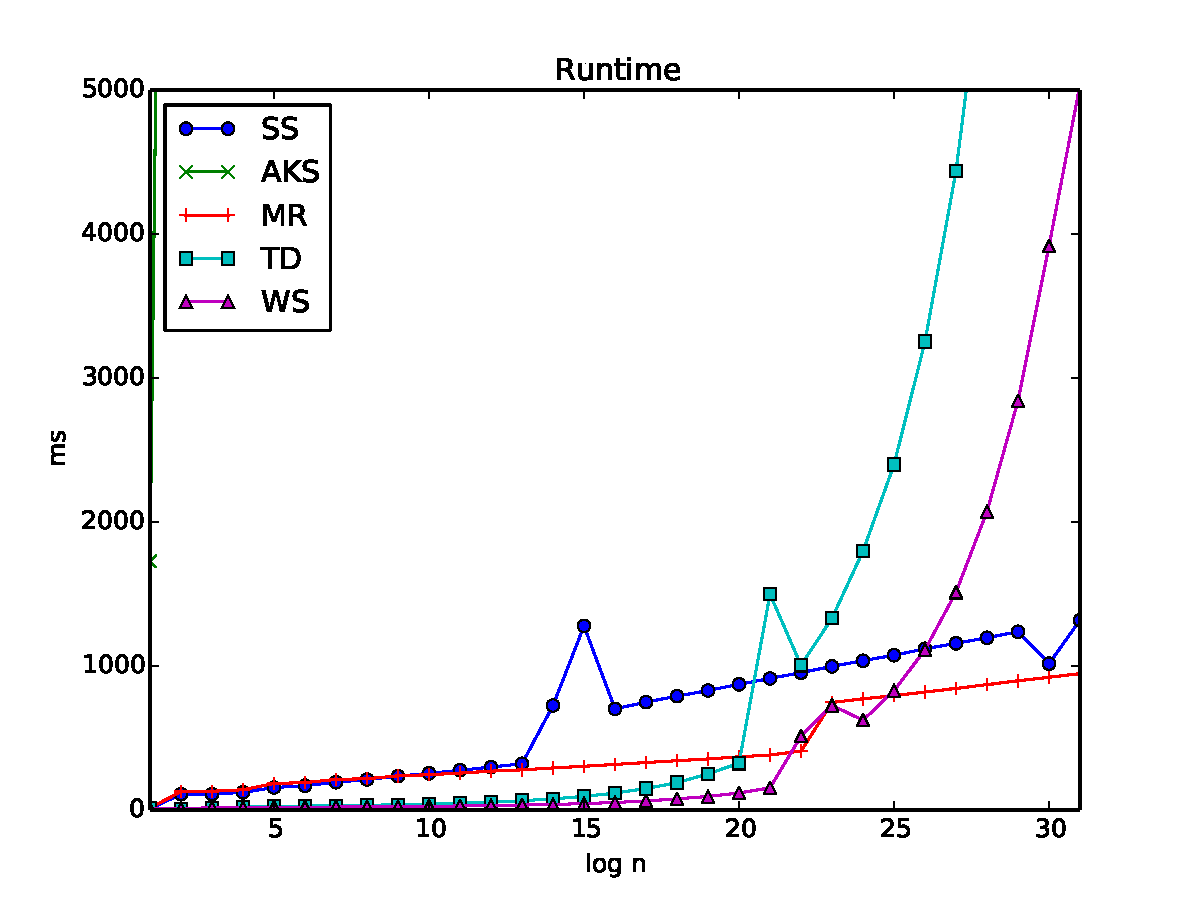
\includegraphics[width=\columnwidth]{results/runtime.pdf}
        \caption{Execution time as function of $\log n$}
        \label{fig:runtime}
\end{figure}

\begin{figure}
        \centering
        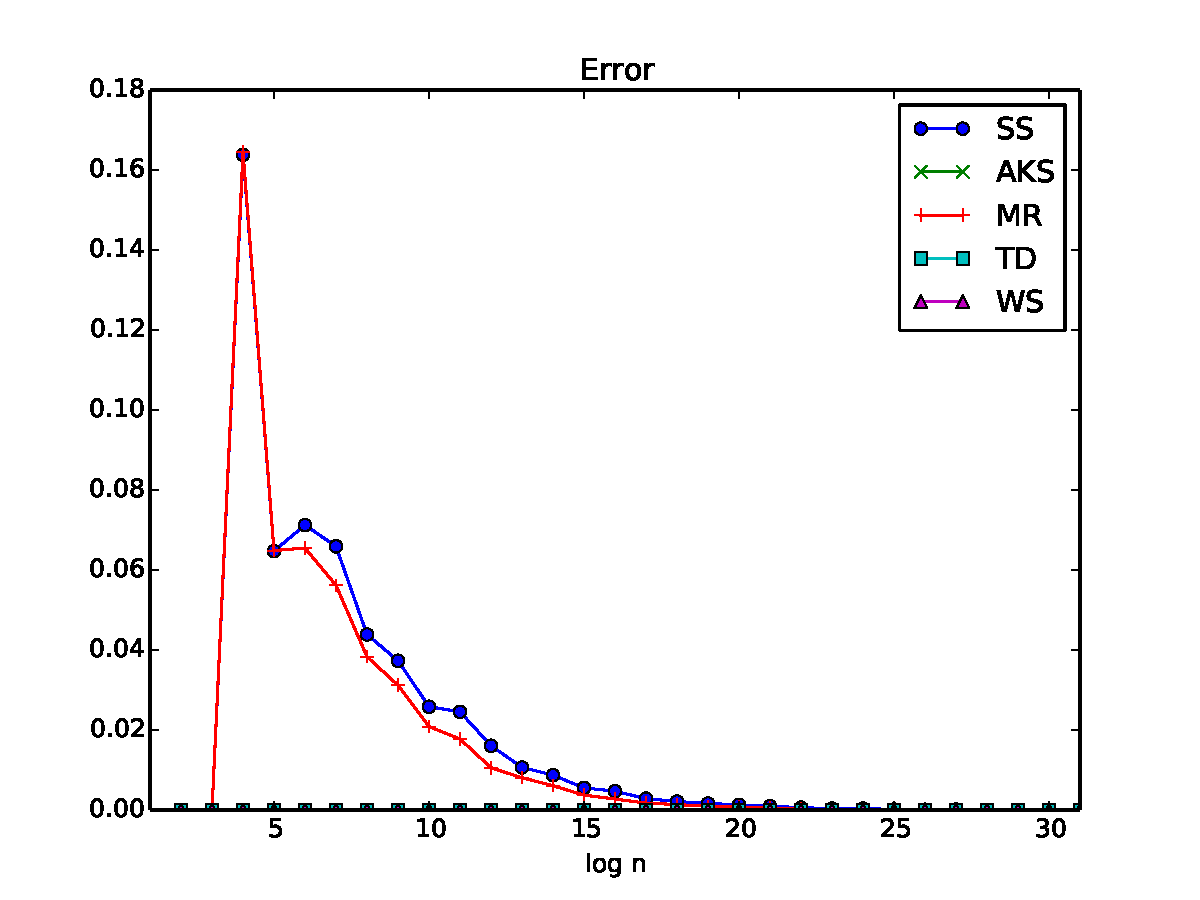
\includegraphics[width=\columnwidth]{results/performance.pdf}
        \caption{Execution time as function of $\log n$}
        \label{fig:results}
\end{figure}




% \begin{table}
% \centering
% \caption{Execution time as a function of $n$. Each datapoint consists of 10,000 samples.}
% \begin{tabular}{|l|c|c|c|c|c|} \hline
% Range\textbackslash Method&AKS&MR&SS&TD&WS \\ \hline
% 2-500&6.55E9&1.86E-2&2.20E-2&3.61E-3&1.06E-2 \\ \hline
% 501-5000&-&1.94E-2&2.52E-2&4.65E-3&1.26E-2 \\ \hline
% 5001-50000&-&2.11E-2&2.82E-2&6.36E-3&1.44E-2 \\ \hline
% 50001-500000&-&2.19E-2&3.15E-2&1.03E-2&1.74E-2 \\ \hline
% \end{tabular}
% \label{tab:pressure}
% \end{table}

\begin{table}
\centering
\caption{Execution time for AKS in the number range 2-500. Each datapoint consists of 10,000 samples.}
\begin{tabular}{|c|c|} \hline
Prime numbers included & $O(10^9)$s\\ \hline
Composite numbers only & $O(1)$s\\ \hline
\end{tabular}
\label{tab:pressure}
\end{table}



%\begin{table}
%\centering
%\caption{Error (fraction) as a function of $n$. Each datapoint consists of 10,000 samples. All methods have a one-sided error: they may say ``prime'', while it is a composite.}
%\begin{tabular}{|l|c|c|c|c|c|} \hline
%Range\textbackslash Method&AKS&MR&SS&TD&WS \\ \hline
%2-500&0&1.27E-2&9.52E-3&0&0 \\ \hline
%501-5000&-&2.64E-3&2.99E-3&0&0 \\ \hline
%5001-50000&-&1.11E-3&5.53E-4&0&0 \\ \hline
%50001-500000&-&1.09E-4&0&0&0 \\ \hline
%\end{tabular}
%\label{tab:pressure}
%\end{table}



%\begin{figure}
        %\centering
        %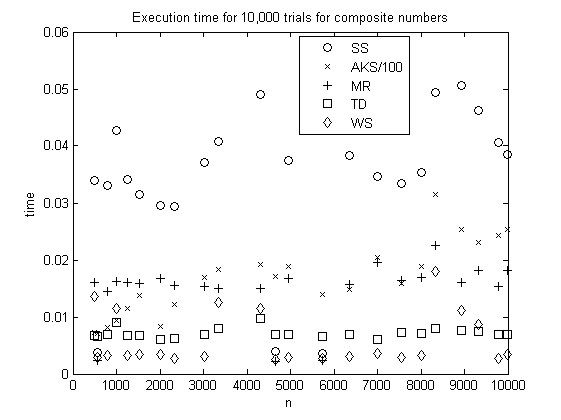
\includegraphics[width=0.5\textwidth]{../Graphs/ExecutionTime1.png}
        %\caption{Execution time for small composite numbers, $n$. Each measurement consists of 10,000 samples.}
        %\label{fig:executionTime1}
%\end{figure}


%\begin{figure}
        %\centering
        %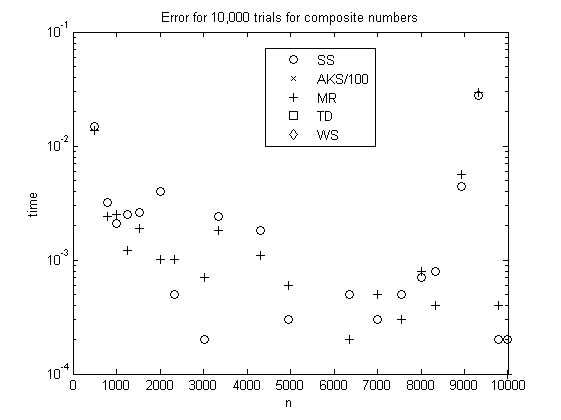
\includegraphics[width=0.5\textwidth]{../Graphs/Error1.png}
        %\caption{Error (false prime prediction) for small composite numbers, $n$. Each measurement consists of 10,000 samples.}
        %\label{fig:error1}
%\end{figure}


%\begin{figure}
        %\centering
        %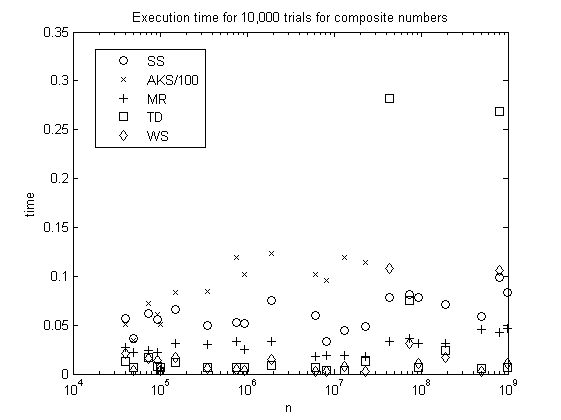
\includegraphics[width=0.5\textwidth]{../Graphs/ExecutionTime2.png}
        %\caption{Execution time for a large range of composite numbers, $n$. Each measurement consists of 10,000 samples.}
        %\label{fig:executionTime2}
%\end{figure}



%\begin{figure}
        %\centering
        %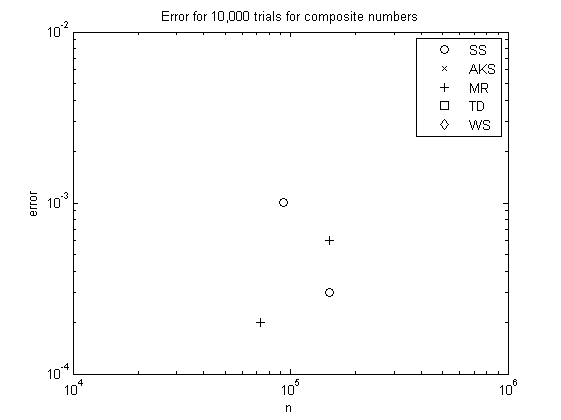
\includegraphics[width=0.5\textwidth]{../Graphs/Error2.png}
        %\caption{Error (false prime prediction) for a large range of composite numbers, $n$. Each measurement consists of 10,000 samples.}
        %\label{fig:error2}
%\end{figure}

